\subsection{Processo di diffusione inversa}


La magia dei modelli di diffusione avviene nel processo di diffusione inversa (\emph{reverse diffusion process}). 
La \emph{ratio} sottesa al processo di diffusione inversa è quella di rimuovere iterativamente rumore
(\emph{denoising}) dall'immagine $\mathbf{x}_T\sim\mathcal{N}(\bm{0},\bm{I})$ (a cui si perviene a valle del processo di diffusione in avanti),
per risalire alla distribuzione incognita dell'immagine di partenza $q(\mathbf{x}_0)$ (Figura~\ref{fig:reverse_diff_process}).
Tuttavia per assolvere a tale scopo, il processo di diffusione inversa non può servirsi della distribuzione a posteriori
$q(\mathbf{x}_{t-1}|\mathbf{x}_t)$. Infatti, ricorrendo alla legge di Bayes~\eqref{eq:Bayes}, risulta che
\begin{equation}
    q(\mathbf{x}_{t-1}|\mathbf{x}_t)=\frac{q(\mathbf{x}_{t}|\mathbf{x}_{t-1})q(\mathbf{x}_{t-1})}{q(\mathbf{x}_t)} \label{eq:reverse_transition}
\end{equation}
da cui si evince come l'intrattabilità di $q(\mathbf{x}_{t-1}|\mathbf{x}_t)$ sia imputabile alle distribuzioni marginali $q(\mathbf{x}_{t-1})$ e $q(\mathbf{x}_t)$ 
in quanto~\footnote{Risultato analogo sussite \emph{mutatis mutandis} per $q(\mathbf{x}_{t-1})$}:
\begin{align}
    q(\mathbf{x}_t) &= \int q(\mathbf{x}_0,\mathbf{x}_1,\dots,\mathbf{x}_t)\,d\mathbf{x}_0\,d\mathbf{x}_1\dots\,d\mathbf{x}_{t-1} \label{eq:marginalization_op} \\
                    &= \int q(\mathbf{x}_1,\dots,\mathbf{x}_t|\mathbf{x}_0)q(\mathbf{x}_0) \,d\mathbf{x}_0\,d\mathbf{x}_1\dots\,d\mathbf{x}_{t-1} \label{eq:marginal}
\end{align}
dove $q(\mathbf{x}_1,\dots,\mathbf{x}_t|\mathbf{x}_0)$ è la catena markoviana della diffusione in avanti definita dalla~\eqref{eq:forward_process}, 
e nella~\eqref{eq:marginalization_op} si è effettuata l'operazione di marginalizzazione~\eqref{eq:marginalizzazione}.

Dalla~\eqref{eq:marginal} si evince chiaramente che il problema sotteso al calcolo di $q(\mathbf{x}_t)$ è duplice:
\begin{itemize}
\item la distribuzione $q(\mathbf{x}_0)$ è \emph{incognita}.
\item l'integrale nella~\eqref{eq:marginal}, essendo esteso ad uno spazio (di pixel) ad alta dimensionalità, è \emph{intrattabile}.
\end{itemize}
\begin{figure}
    \centering
    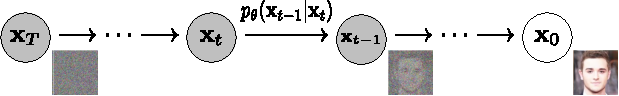
\includegraphics[keepaspectratio]{reverse_diff_process}
    \caption{Processo di diffusione inversa. Fonte:~\cite{ho2020}.}
    \label{fig:reverse_diff_process}
\end{figure}
Ho et al.~\cite{ho2020}, sulla scia di Sohl-Dickstein et al.~\cite{sohl-dickstein2015}, propongono l'addestramento di una rete neurale
per approssimare $q(\mathbf{x}_{t-1}|\mathbf{x}_t)$.

\noindent Il processo di diffusione inversa, quindi, è definito come un catena markoviana di transizioni gaussiane i cui parametri
(i.e.\ media e varianza) sono appresi 
da una rete neurale. L'assunzione di gaussianità per le suddette transizioni è supportata 
dall'osservazione che, qualora i $\beta_t$ abbiano entità contenuta, le transizioni di entrambi i processi 
di diffusione (diretta e inversa) esibiscono la stessa forma funzionale~\cite{fellerTheoryStochasticProcesses1949}.
Matematicamente risulta che:
\noindent 
\begin{Mybox1}
\begin{gather}
    p_{\bm{\theta}}(\mathbf{x}_{0:T})   \triangleq p(\mathbf{x}_T)\prod\limits_{t=1}^{T}p_{\bm{\theta}}(\mathbf{x}_{t-1}|\mathbf{x}_t) \, \text{Processo di diffusione inversa} \label{eq:reverse_process} \\
    p_{\bm{\theta}}(\mathbf{x}_{t-1}|\mathbf{x}_t) \triangleq \mathcal{N}(\mathbf{x}_{t-1}; \bm{\mu}_{\bm{\theta}}(\mathbf{x}_t,t),\bm{\Sigma}_{\bm{\theta}}(\mathbf{x}_t,t)) \,  \text{Generica transizione}\label{eq:chain_transition132}
\end{gather}
\end{Mybox1}
\noindent dove:
\begin{itemize}
\item $p(\mathbf{x}_T)=q(\mathbf{x}_T)=\mathcal{N}(\mathbf{x}_T;\bm{0},\bm{I})$ dal momento 
che il punto di arrivo della diffusione in avanti costituisce la base di partenza del processo di diffusione inversa.
\item il pedice $\bm{\theta}$ denota il vettore dei \emph{parametri} della rete neurale, aggiornati con la tecnica del gradiente discendente stocastico.
\item $\bm{\mu}_{\bm{\theta}}(\mathbf{x}_t,t)$,$\bm{\Sigma}_{\bm{\theta}}(\mathbf{x}_t,t)$ 
sono rispettivamente media e varianza che, come suggerisce la notazione (i.e il pedice $\bm{\theta}$), sono appresi dalla rete neurale.
\end{itemize}

\bigskip
\noindent Ricapitolando, il processo di diffusione inversa consiste nel rimuovere 
iterativamente (anziché in un singolo passo come le GAN~\cite{changDesignFundDiffusion2023}), servendosi di una rete neurale, 
il rumore dall'immagine $\mathbf{x}_T$. Tale processo di diffusione inversa è imbastito sull'immagine terminale della diffusione in avanti
e, al decrescere di $t$ da $T$ a $0$, si propaga nella direzione opposta a quest'ultima tramite una catena markoviana 
di transizioni~\eqref{eq:chain_transition132}.